\documentclass{beamer}
\usepackage[utf8]{inputenc}
\usepackage[T2A,T1]{fontenc}
\usepackage[english, russian]{babel}
\usetheme{Pittsburgh}

\selectlanguage{russian}
\newcommand{\define}[2]{{\bf #1} --- #2.\vspace{1em}}
\newcommand{\longdef}[1]{{\textbf{\underline{Опр:}} #1}}
%Add identation from the left side for theorema text
\newcommand{\theorema}[1]{{\textbf{\underline{Теор:}} #1}}
\newcommand{\set}[1]{{\lbrace #1 \rbrace}}

\title{МАС на основе криптографических хеш-функций}
\institute{ВГУ}
\date{2014}
\begin{document}

\frame{\titlepage}

\begin{frame}
  \frametitle{Классификация криптографических алгоритмов}

  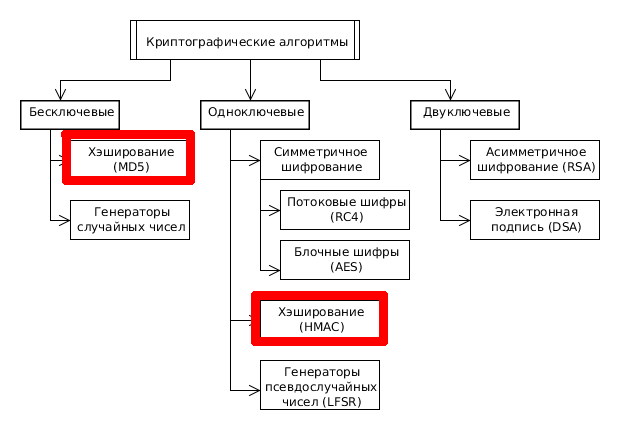
\includegraphics[width=\linewidth]{./images/png/CA_classification_hash_func.png}

\end{frame}

\begin{frame}
  \frametitle{Стойкость к коллизиям}

  Пусть $H: M \rightarrow T$ некоторая хеш-функция $(|M| \gg |T|)$

  \vspace{8mm}

  \underline{Коллизией} для $H$ называется пара $m_{0}, m_{1} \in M$ такая, что:
  \[ H(m_0) = H(m_1), m_0 \neq m_1 \]

  \vspace{8mm}

  Функция $H$ является \underline{стойкой к коллизиям}, если для всех эффективно
  вычислимых алгоритмов $A$ вероятность того, что алгоритм $A$ найдет
  коллизию для функции $H$ пренебрежительно мала.

  \vspace{8mm}

  Пример: SHA-256
\end{frame}

\begin{frame}
  \frametitle{MAC из стойкой к коллизиям хеш-функции}

  Пусть $I=(S,V)$ -- MAC для коротких сообщений над $(K,M,T)$
  Пусть $H:M^{big} \rightarrow M$

  \vspace{8mm}

  Определим $I^{big} = (S^{big}, V^{big})$ над $(K, M^{big}, T)$ как:
  \[ S^{big}(k,m) = S(k, H(m));\]
  \[ V^{big}(k,m) = V(k, H(m), t)\]

\end{frame}

\begin{frame}
  \frametitle{MAC из стойкой к коллизиям хеш-функции}

  \theorema{Если $I$ -- безопасный MAC и $H$ - стойкая к коллизиям хеш-функция, то
            $I^{big}$ тоже является безопасным MAC}

  \vspace{10mm}

  Пример:  $S(k,m) = AES_{2-block-CBC}(k, \text{SHA-256}(m))$

  \vspace{8mm}
  Если для хеш-функции находится коллизия, то MAC становится небезопасным
\end{frame}

\begin{frame}
  \frametitle{Обеспечение целостности файлов}

  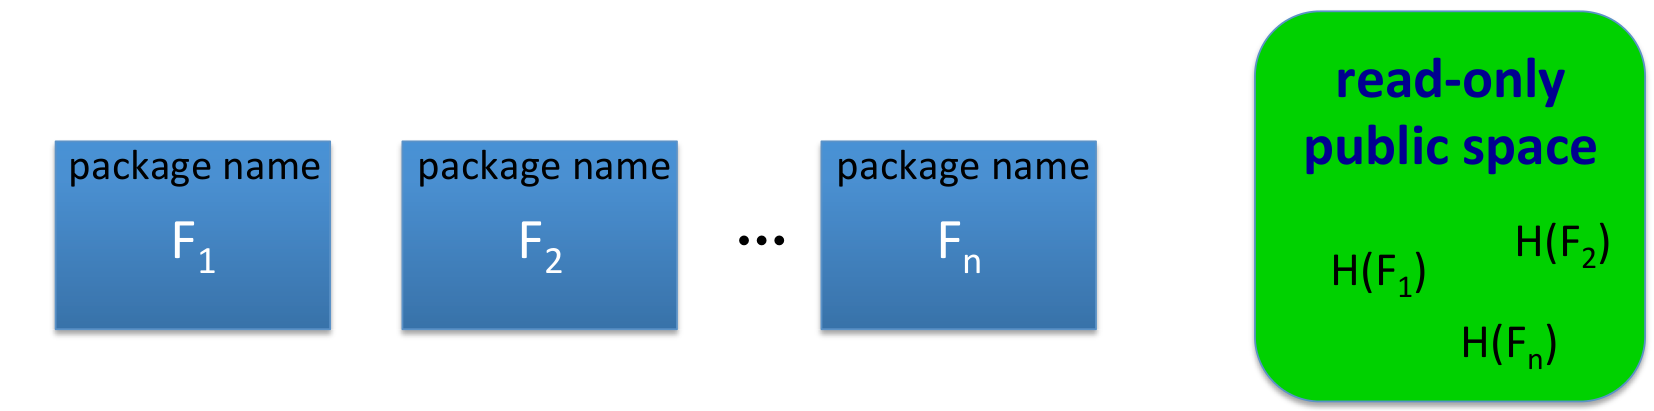
\includegraphics[width=\linewidth]{./images/png/CR_hash_packages.png}
  \begin{itemize}
    \item{Пользователь при скачивании пакета может проверить его целостность, посчитав $H(F)$}
    \item{Злоумышленник не может подменить пакет, оставшись незамеченным}
    \item{Нет необходимости в секретном ключе. Единственное требование - защищенное хранилище для хешей пакетов}
  \end{itemize}
\end{frame}

\begin{frame}
  \frametitle{Парадокс ``дней рождения``}

  Пусть $r_1, r_2, \ldots, r_n \in \set{1,\ldots,B}$ -- независимые одинаково распределенные случайные целые числа.

  \vspace{4mm}
  \theorema{Если $n=1.2 \times B^{1/2}$, то $P[ \exists i \neq j: r_i = r_j ] \geq 1/2$}

  \vspace{4mm}
  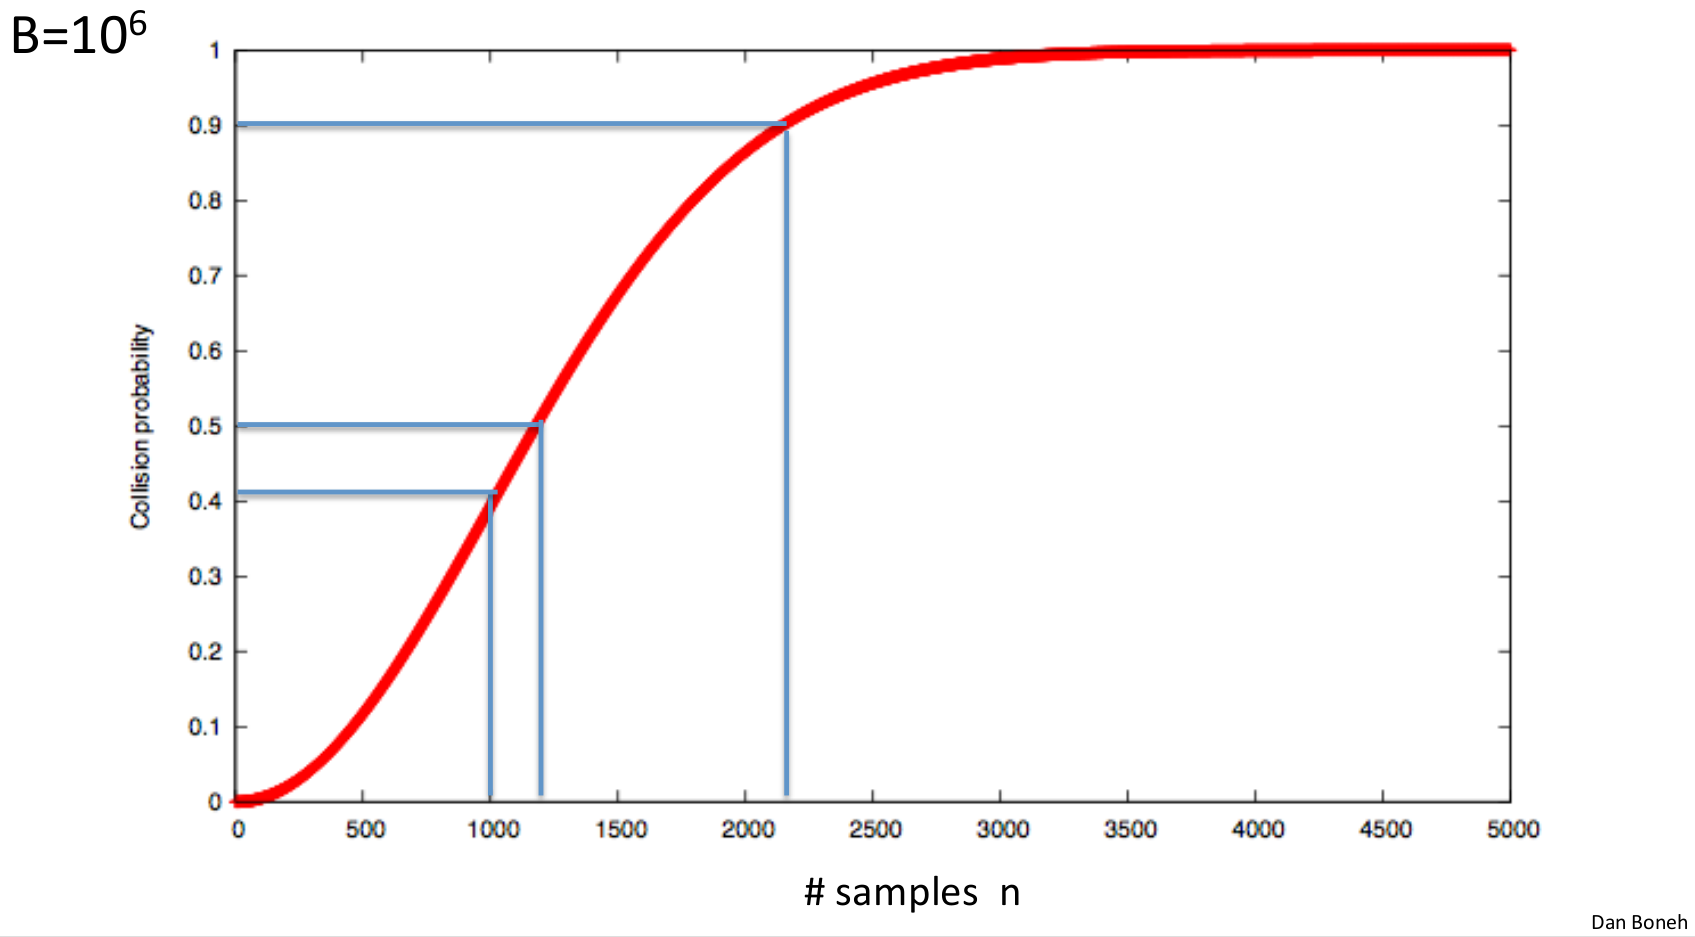
\includegraphics[width=100mm]{./images/png/birthday_paradox.png}
\end{frame}

% TODO: Add frame with generic birthday attack algo

\begin{frame}
  \frametitle{Построение стойкой к коллизиям хеш-функции}

  \begin{block}{Основная идея}
  Имея стойкую к коллизиям хеш-функцию для \underline{коротких}
  сообщений, построить стойкую к коллизиям хеш-функцию для \underline{длинных}
  сообщений.
  \end{block}
\end{frame}

\begin{frame}
  \frametitle{Построение стойкой к коллизиям хеш-функции}

  \begin{block}{Основная идея}
  Имея стойкую к коллизиям хеш-функцию для \underline{коротких}
  сообщений, построить стойкую к коллизиям хеш-функцию для \underline{длинных}
  сообщений.
  \end{block}

  \vspace{8mm}
  Этот подход реализует метод построения, называемый \underline{конструкцией Меркла-Дамгарда}.
\end{frame}

\begin{frame}
  \frametitle{Конструкция Меркла-Дамгарда}

\end{frame}

\end{document}
